This section describes the generative model learning. We employ a method \cite{kopicki2015ijrr}, which learns a generative model of a dexterous grasp from a demonstration (LfD). That paper posed it as the problem of learning a factored probabilistic model. The method is split into a model learning phase, a model transfer phase, and the grasp generation phase. 

\subsection{Model learning}
The model learning is split into three parts: acquiring an {\em object model}; using this object model, with a demonstrated grasp, to build a {\em contact model} for each finger link in contact with the object; and acquiring a {\em hand configuration model} from the demonstrated grasp. After learning the object model can be discarded.

\subsubsection{Object model}
First, a point cloud of the object used for the demonstrated grasp is acquired by a depth camera, from several views. Each point is augmented with the estimated principal curvatures at that point and a surface normal. Thus, the $j^{th}$ point  in the cloud gives rise to a feature $x_j=(p_j, q_j, r_j)$, with the components being its position $p_j \in \mathbb R^3$, orientation $q_j \in SO(3)$ and principal curvatures $r_j=(r_{j,1},r_{j,2}) \in \mathbb R^2$. The orientation $q_j$ is defined by $k_{j,1},k_{j,2}$, which are the directions of the principal curvatures.  For later convenience we use $v=(p,q)$ to denote position and orientation combined. These features $x_j$ allow the object model to be defined as a kernel density estimate of the joint density over $v$ and $r$.
\begin{equation}
\om(v, r) \equiv \pdf^\om(v, r) \simeq \sum_{j=1}^{K_O} w_j \mathcal{K}(v, r|{x_j}, \sigma_{x})
%RD: mu and sigma are not properly defined.
\label{eq:om}
\end{equation}
where $\om$ is short for $\pdf^\om$, bandwidth $\sigma_{x} = (\sigma_{p}, \sigma _{q}, \sigma_{r})$, $K_O$ is the number of features $x_j$ in the object model, all weights are equal $w_j = 1/{K_O}$, and $\mathcal{K}$ is defined as a product:
\begin{equation}\label{eq:kernel_in_se3}
\mathcal{K}(x | \mu, \sigma) = \mathcal{N}_3(p| \mu_p, \sigma_p) \Theta(q| \mu_q, \sigma_q) \mathcal{N}_2(r| \mu_r, \sigma_r)
\end{equation}
where $\mu$ is the kernel mean point, $\sigma$ is the kernel bandwidth, $\mathcal{N}_n$ is an $n$-variate isotropic Gaussian kernel, and ${\Theta}$ corresponds to a pair of antipodal von Mises-Fisher distributions.
\begin{figure*}[t]
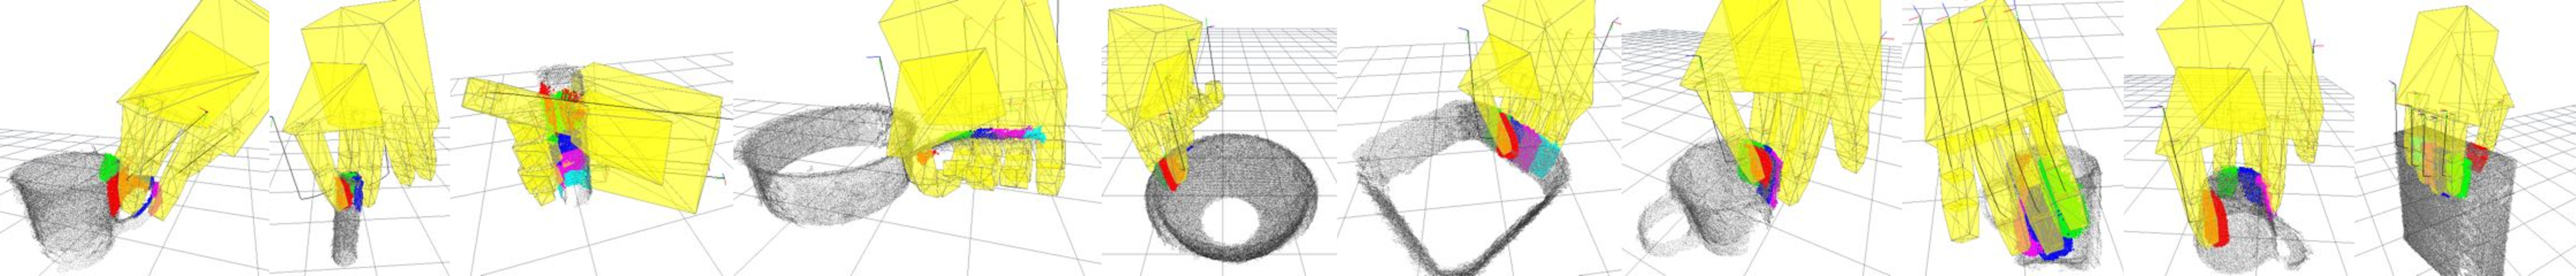
\includegraphics[width=\textwidth]{images/training-examples}
%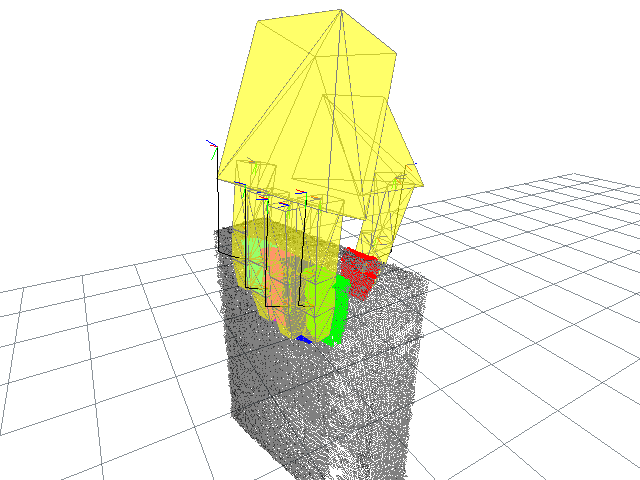
\includegraphics[width=0.1\textwidth]{images/contact-viewall2}
%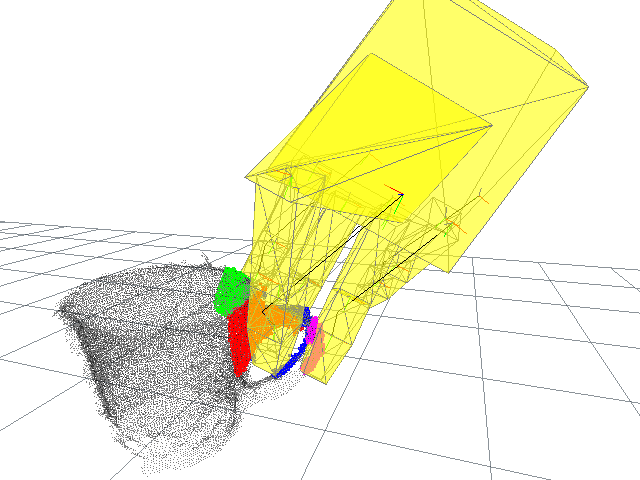
\includegraphics[width=0.1\textwidth]{images/contact-viewall3}
%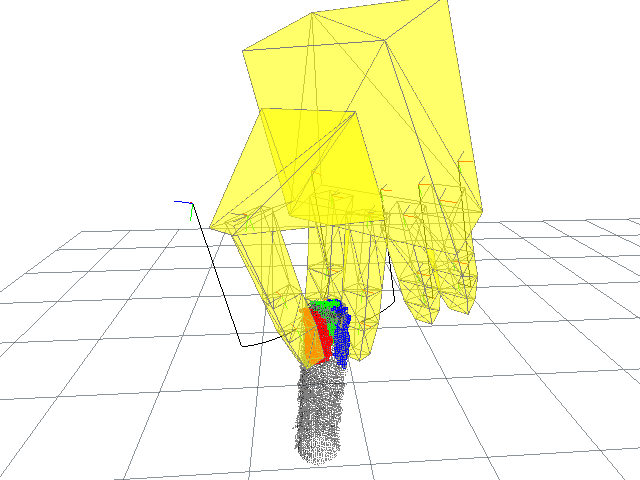
\includegraphics[width=0.1\textwidth]{images/contact-viewall4}
%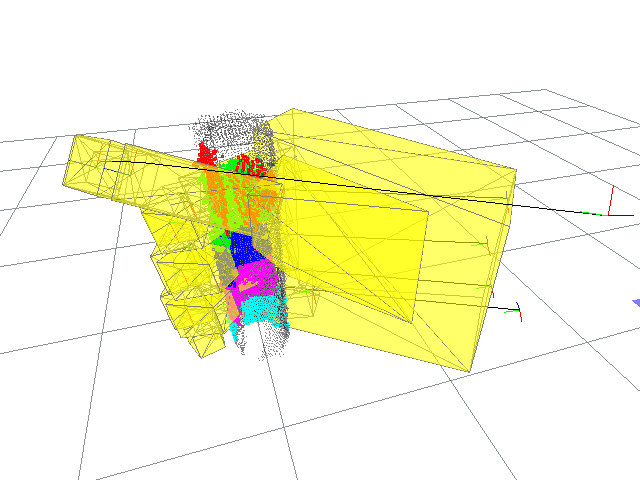
\includegraphics[width=0.1\textwidth]{images/contact-viewall5}
%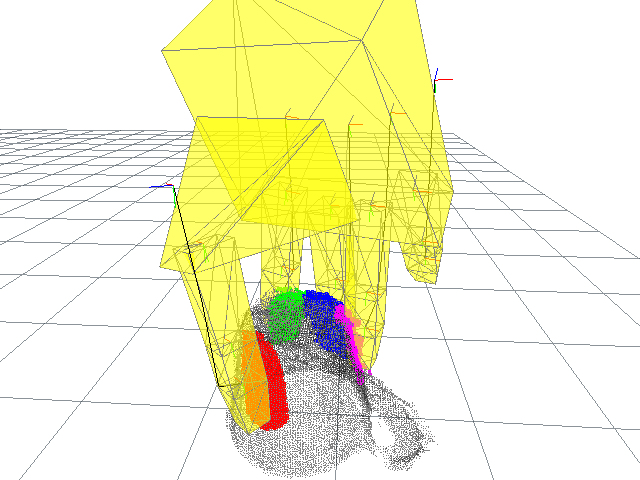
\includegraphics[width=0.1\textwidth]{images/contact-viewall6}
%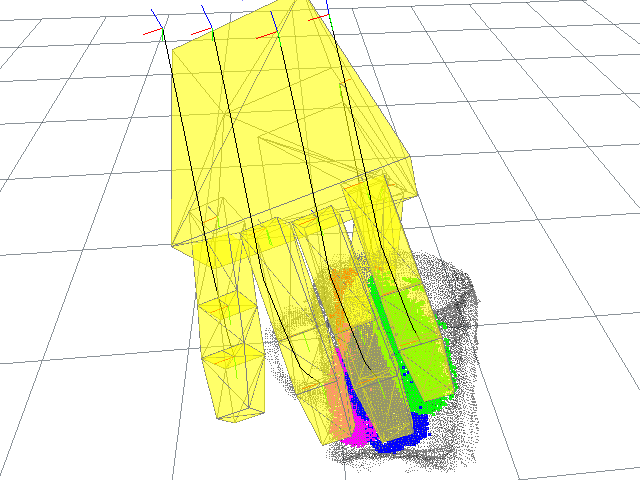
\includegraphics[width=0.1\textwidth]{images/contact-viewall7}
%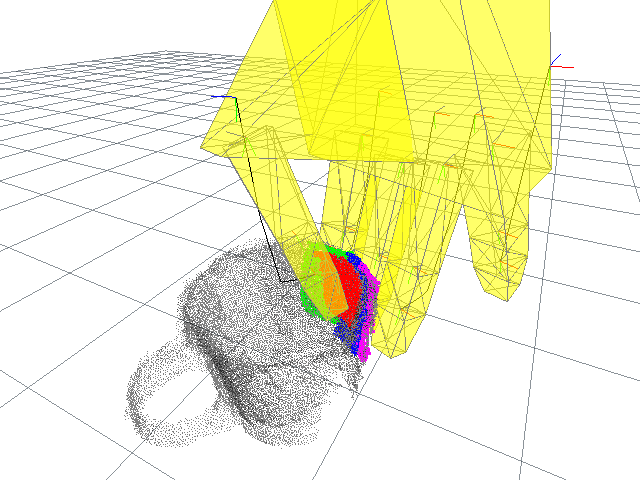
\includegraphics[width=0.1\textwidth]{images/contact-viewall8}
%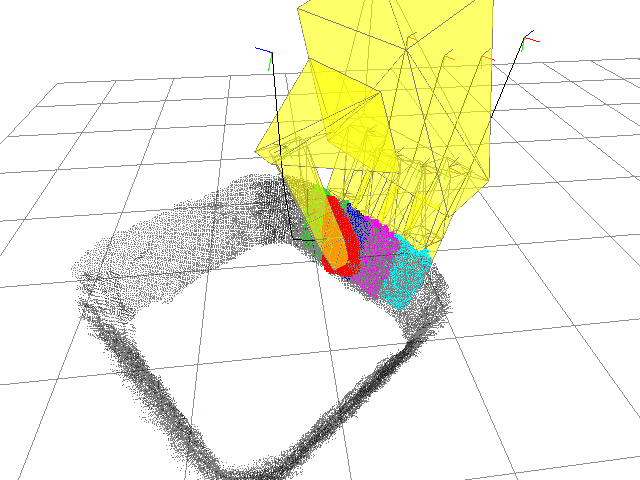
\includegraphics[width=0.1\textwidth]{images/contact-viewall9}
%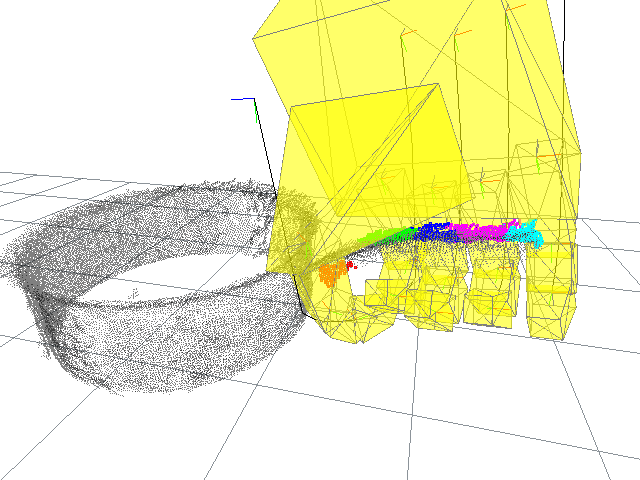
\includegraphics[width=0.1\textwidth]{images/contact-viewall10}
\caption{The ten training grasps for the generative model. The final hand pose is shown in yellow, the sensed point cloud in black, and the parts of the point cloud that contribute to each contact model are coloured by the associated link. \label{fig:generative-training}}
\end{figure*}
\subsubsection{Contact models}
When a grasp is demonstrated the final hand pose is recorded. This is used to find all the finger links $L$ and surface features $x_j$ that are in close proximity. A contact model $M_i$ is built for each finger link $i$. Each feature in the object model that is within some distance $\delta_i$ of finger link $L_i$ contributes to the contact model $\cm_i$ for that link. This contact model is defined for finger link $i$ as follows:
\begin{equation}
\cm_i(u, r) \equiv \pdf^\cm_i(u, r) \simeq \frac{1}{Z} \sum_{j=1}^{K_{M_i}} w_{ij} \mathcal{K}(u, r | {x_j}, \sigma_{x})
%RD: mu and sigma are not properly defined.
\label{eq:cm}
\end{equation}
where $u$ is the pose of $\rl_i$ relative to the pose $v_j$ of the $j^{\mathnormal{th}}$ surface feature, $K_{M_i}$ is the number of surface features in the neighbourhood of link $L_i$, $Z$ is the normalising constant, and $w_{ij}$ is a weight that falls off exponentially as the distance between the feature $x_j$ and the closest point $a_{ij}$ on finger link $L_i$ increases:
\begin{equation}
w_{ij} = \begin{cases}\exp(-\lambda ||p_j-a_{ij}||^2) \quad &\textnormal{ if } ||p_j-a_{ij}|| < \delta_i\\
0 \quad &\textnormal{ otherwise},\end{cases}
\label{eq:learning.modeldist.wgh}
\end{equation}
The key property of a contact model is that it is conditioned on local surface features likely to be found on other objects, so that the grasp can be transferred. We use the principal curvatures $r$, but many local surface descriptors would do. %A contact model can be visualised by marginalising out the dimensions for the rigid body transformation $u$, showing us the distribution over the local curvatures that finger link $L_i$ experienced in the demonstrated grasp. 
%
%\begin{figure*}
%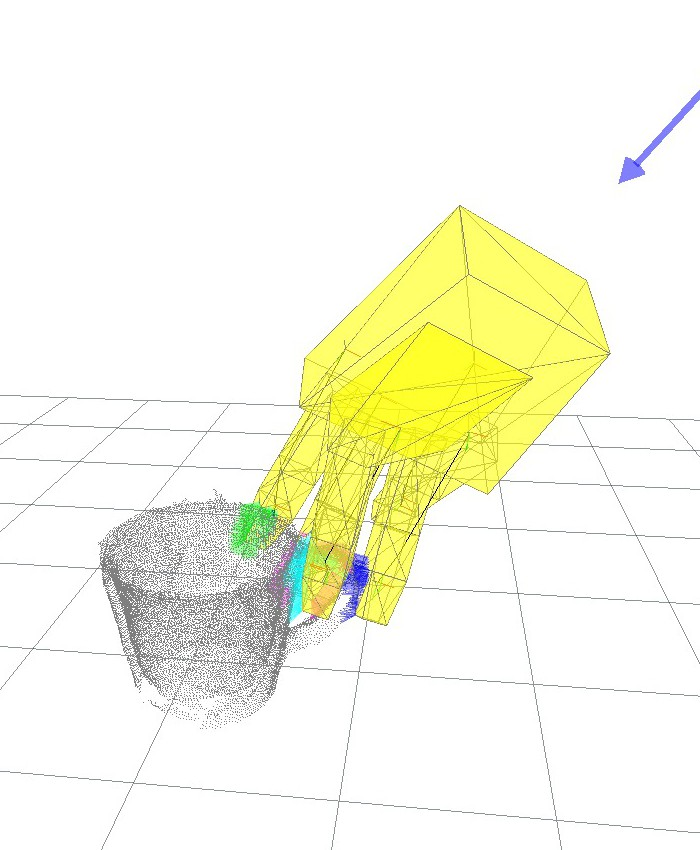
\includegraphics[height=2cm]{images/contact-model-learning/handle-grasp}
%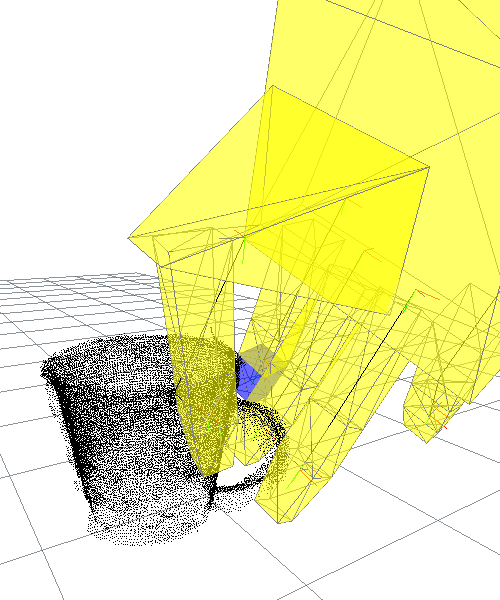
\includegraphics[height=2cm]{images/contact-model-learning/link8}
%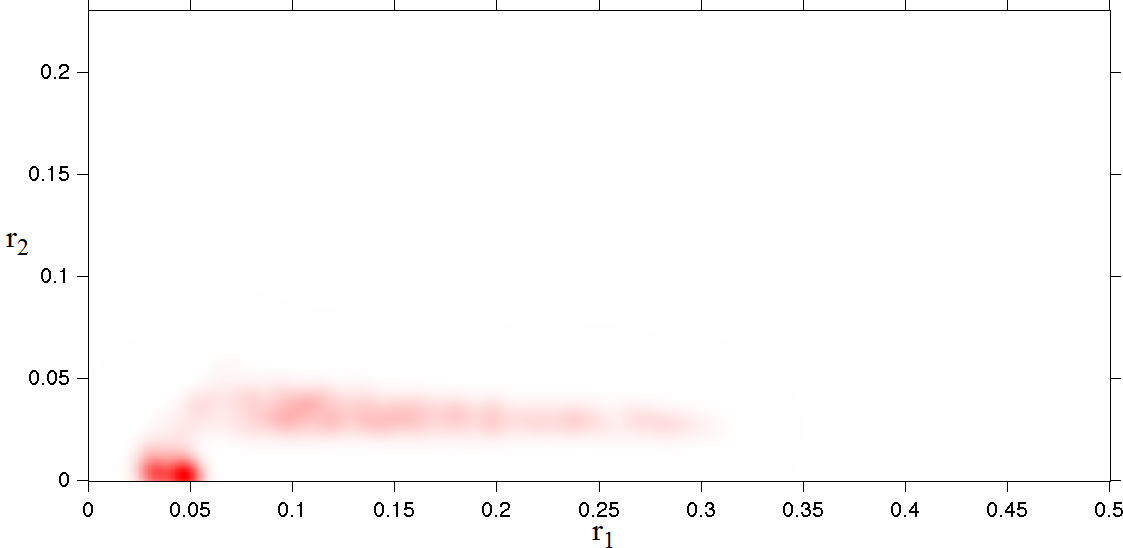
\includegraphics[height=2cm]{images/contact-model-learning/handle_model_08_00778r}
%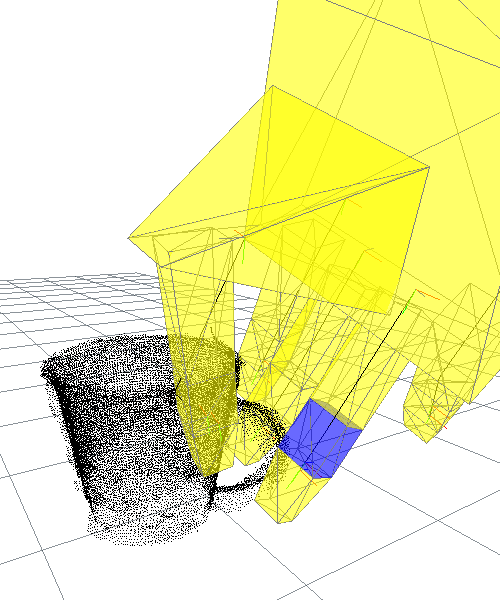
\includegraphics[height=2cm]{images/contact-model-learning/link15}
%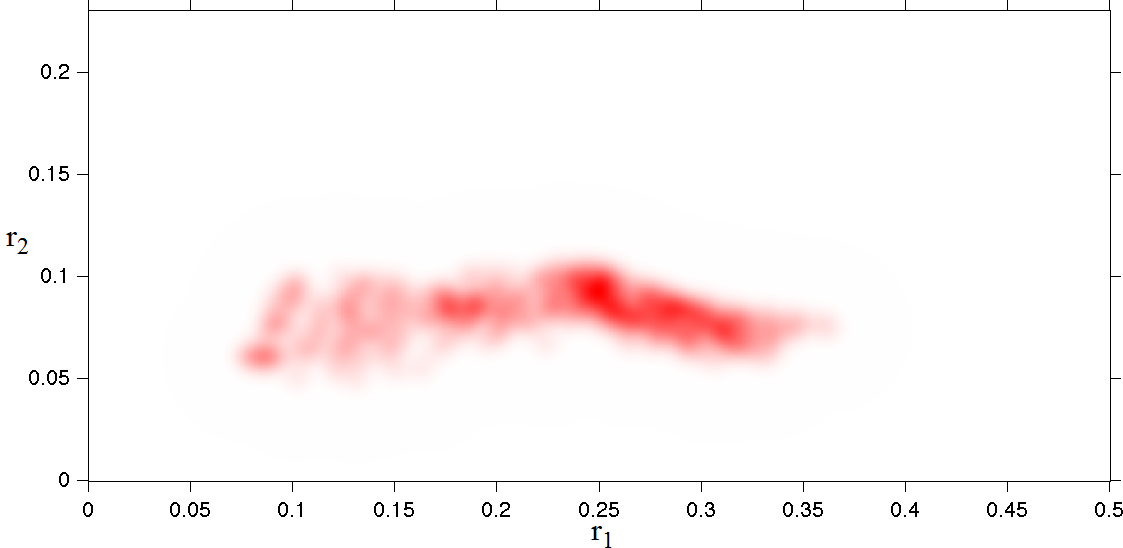
\includegraphics[height=2cm]{images/contact-model-learning/handle_model_15_00329r}
%  \caption{A training grasp and some contact models arising from it.}
%  \label{fig:contactModels}
%\end{figure*}

\subsection{Hand configuration model}
In addition to a contact model for each finger-link, a model of the hand configuration $h_c \in \mathbb R^D$ is recorded, where $D$ is the number of DoF in the hand. $h_c$  is recorded for several points on the demonstrated grasp trajectory as the hand closed. The learned model is:
\begin{equation}
\hc(h_c) \equiv \sum_{\gamma \in [-\beta, \beta]} w({h_c(\gamma)}) \mathcal{N}_D(h_c|h_c(\gamma), \sigma_{h_c}) 
\label{eq:hc}
\end{equation}
where $w({h_c(\gamma)}) = \exp(-\alpha \|h_c(\gamma) - h^g_c \|^2)$; $\gamma$ is a parameter that interpolates between the beginning ($h^t_c$) and end ($h^g_c$) points on the trajectory, governed via \eq\ref{eq:learning.configmodel.config} below; and $\beta$ is a parameter that allows extrapolation of the hand configuration.
\begin{equation}
h_c(\gamma) = (1 - \gamma)h^g_c + \gamma h^t_c
\label{eq:learning.configmodel.config}
\end{equation}
\subsection{Grasp Transfer}
When presented with a new object $o_{new}$ the contact models must be transferred to that object. A partial point cloud of $o_{new}$ is acquired (from a single view) and recast as a density, $\om_{new}$, again using \eq \ref{eq:om}. The transfer of each contact model $\cm_i$ is achieved by convolving $\cm_i$ with $\om_{new}$. This convolution is approximated with a Monte-Carlo method, resulting in an kernel density model of the pose $s$ of the finger link $i$ (in workspace coordinates) for the new object. The Monte-Carlo procedure samples poses for link $L_i$ on the new object. The $j^{th}$ sample is $\hat{s}_{ij}=(\hat{p}_{ij},\hat{q}_{ij})$. Each sample $\hat{s}_{ij}$ is weighted $w_{ij}$ by its likelihood. These samples are used to build what we term the query density:
\begin{equation}
\qd_i(s) \simeq \sum^{K_{Q_i}}_{j=1} w_{ij} \mathcal{N}_3(p|{\hat{p}_{ij}}, \sigma_{p}) \Theta(q|{\hat{q}_{ij}}, \sigma_{q})%, \quad i = 1, ..., N_L
\label{eq:qd.approx}
\end{equation}
where all the weights are normalised, $\sum_j w_{ij} = 1$. A query density is constructed for every contact model and the new object. These query densities, together with the hand configuration model, are then used to generate grasps. Query density computation is fast, taking $<0.5s$  per grasp model.
\begin{figure*}[t]
\begin{center}
  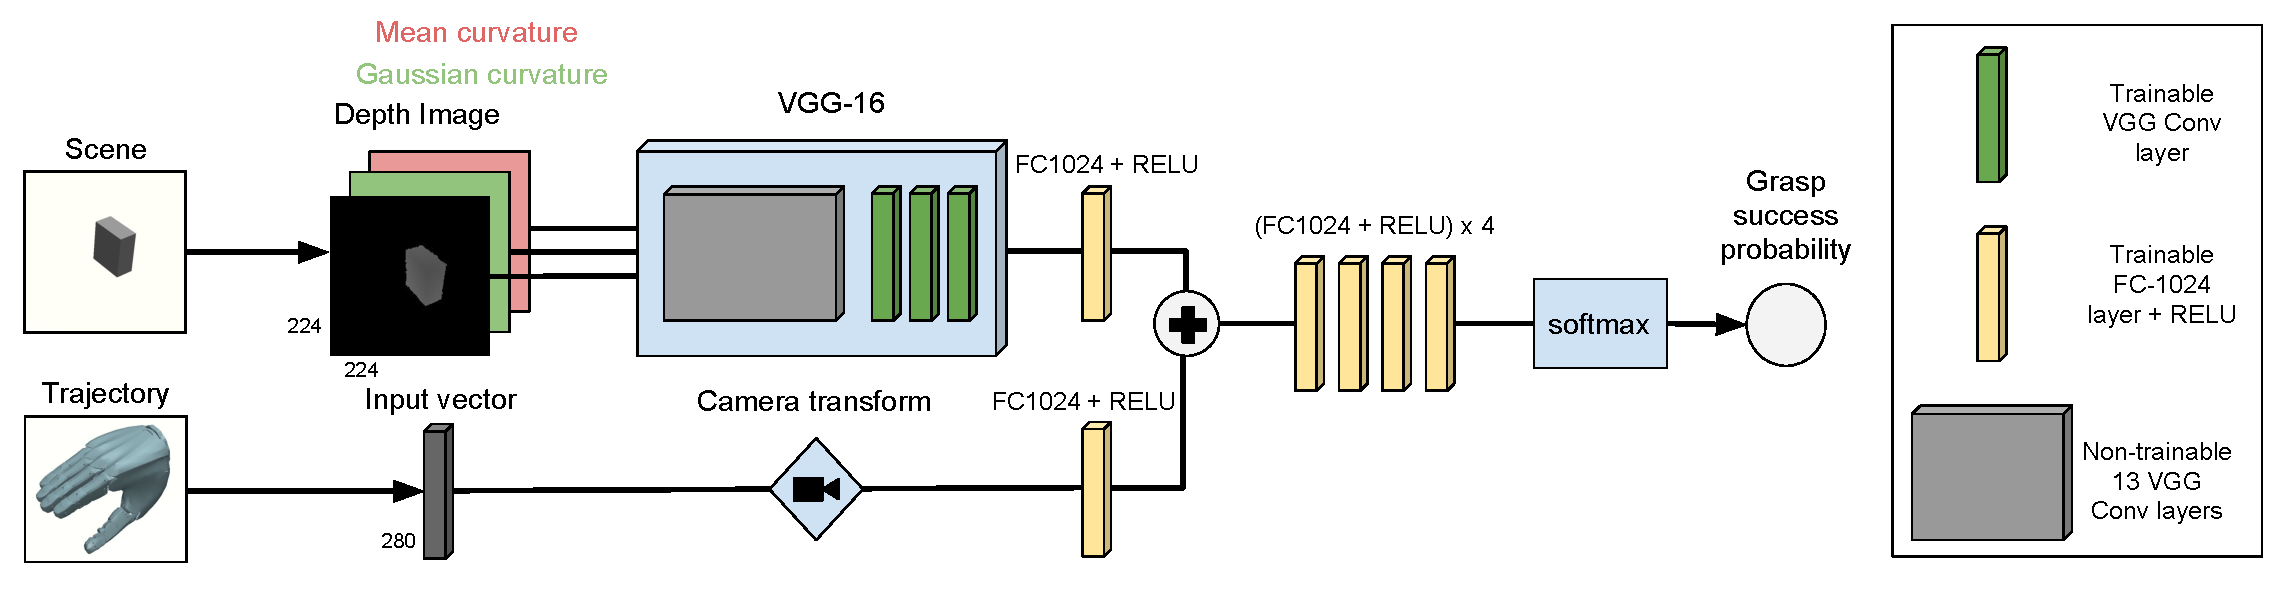
\includegraphics[width=0.85\textwidth]{images/networkArchitecture.pdf}
  \end{center}
  \caption{The evaluative network architecture.}
\label{fig:networkArchitecture}
\end{figure*}
\subsection{Grasp generation}
Candidate grasps may be generated as follows. Select a query density $k$ and take a sample  $s_k \sim \qd_{k}$. Then, take a sample $h_c \sim C$ from the hand configuration model. This pair of samples together define, via the hand kinematics, a complete grasp $h=(h_w,h_c)$, where $h_w$ is the pose of the wrist and $h_c$ is the configuration of the hand. The initial grasp is then improved by stochastic hill-climbing on a product of experts:
\begin{equation}
\argmax{(h_w, h_c)} \hc(h_c) \prod_{\qd_i \in \mathcal{Q}} \qd_i\left(k_{i}^{\mathrm{for}}\left(h_w, h_c\right)\right)
\label{eq:grasping.product}
\end{equation}
This generate and improvement process has periodic pruning steps, in which only the higher likelihood grasps are retained. It can be run many times, thus enabling the generation of many candidate grasps. In addition, a separate generative model can be learned for each demonstrated grasp. Thus, when presented with a new object, each grasp model can be used to generate and improve grasps. We generate and optimise 100 grasps per grasp type. Finally, the many candidate grasps generated from each grasp model can be compared and ranked according to their likelihoods. The product of experts formulation, however, only ensures that the generated grasps have high likelihood according to the model. There is no estimate of the probability that the grasp will succeed. This motivates the dual architecture in this paper. We now turn to the learning method we used to re-rank the grasps according to predicted success probability. 

\subsection{Training Grasps for the Evaluative Model}

For this study, ten example grasps were provided (Figure~\ref{fig:generative-training}). In contrast to \cite{kopicki2015ijrr}, although seven views of each training object were taken, we trained a separate generative model for each view. This led to a total of 70 generative models being learned, one for each grasp-view combination. Because of this view based training, we filter surface normals on the object model so that for each contact model we only consider points on the object surface with surface normals within +/- 90 degrees of the surface of the finger link. %Second, rather than globally selecting the best grasps regardless of the training grasp type---as in \cite{kopicki2015ijrr}---we select half globally and half we force to be evenly spread across the grasp types. This keeps a broad range of grasp options open for evaluation.
